\section{Preliminaries} \label{sec:preliminaries}



In this section, we first  define taxonomy, including
hypernym and hyponym. Subsequently,
we discuss challenges of processing taxonomy-based approximate string joins.


\subsection{Taxonomy}

A taxonomy (T ,$\sqsubset$ ) consists of a universe of terms T and
a term-term hypernym-hyponym relationship $\sqsubset$.

Hypernym-hyponym relationship. The hypernym-hyponym relationship
$\sqsubset$ is a partial order T . For two terms t1 and t2,
we write t1 $\sqsubset$ t2 or t2 $\sqsubset$ t1, if t1 is a hypernym of t2 (or t2
is a hyponym of t1). For example, ``Caribbean Region'' is a hyponym of
``Americas''. Figure  \ref{fig:taxonomy} shows an example of taxonomy for geological locations.



Hyponymy shows the relationship between the more general terms (hypernyms) and the more specific instances of it (hyponyms). A hyponym is a word or phrase whose semantic field is more specific than its hypernym. The semantic field of a hypernym, also known as a superordinate, is broader than that of a hyponym. An approach to the relationship between hyponyms and hypernyms is to view a hypernym as consisting of hyponyms. This, however, becomes more difficult with abstract words such as imagine, understand and knowledge. While hyponyms are typically used to refer to nouns, it can also be used on other parts of speech. Like nouns, hyponyms in verbs are words that refer to a broad category of actions. For example, verbs such as stare, gaze, view and peer can also be considered hyponyms of the verb look.
Hypernyms and hyponyms are asymmetric. Hyponymy can be tested by substituting X and Y in the sentence ``X is a kind of Y'' and determining if it makes sense.[4] For example, ``A screwdriver is a kind of tool''  makes sense but not ``A tool is a kind of screwdriver''.


Hyponymy is a transitive relation, if X is a hyponym of Y, and Y is a hyponym of Z, then X is a hyponym of Z.[5] For example, violet is a hyponym of purple and purple is a hyponym of color; therefore violet is a hyponym of color. In addition, it should be noted that a word can be both a hypernym and a hyponym: for example purple is a hyponym of colour but itself is a hypernym of the broad spectrum of shades of purple between the range of crimson and violet.

The hierarchical structure of semantic fields can be mostly seen in hyponymy. They could be observed from top to bottom, where the higher level is more general and the lower level is more specific. For example, living things will be the highest level followed by plants and animals, and the lowest level may comprise dog, cat and wolf.

Under the relations of hyponymy and incompatibility, taxonomic hierarchical structures too can be formed. It consists of two relations; the first one being exemplified in 'An X is a Y' (simple hyponymy) while the second relation is 'An X is a kind/type of Y'. The second relation is said to be more discriminating and can be classified more specifically under the concept of taxonomy.

Computer science often terms this relationship an ``is-a'' relationship. For example, the phrase ``Red is-a colour'' can be used to describe the hyponymic relationship between red and colour.

Hyponymy is the most frequently encoded relation among synsets used in lexical databases such as WordNet. These semantic relations can also be used to compare semantic similarity by judging the distance between two synsets and to analyse Anaphora.

As a hypernym can be understood as a more general word than its hyponym, the relation is used in semantic compression by generalization to reduce a level of specialization.

%\begin{figure}[t]
%\centering
%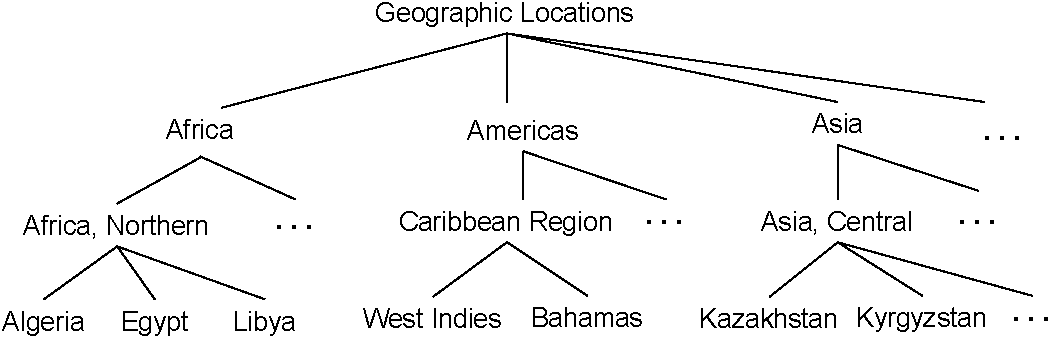
\includegraphics[width=0.45\textwidth]{figures/taxonomy}
% \caption{An example of taxonomy on ``\textsf{Geographic locations}''}
%\label{fig:taxonomy}
%\end{figure}
%
%Example extended SQL
%
%Select  T1.price, T2.price \\
%From Table T1 and T2 \\
%Where T1.area is\_a\_hypernym T2.area \\
%With taxonomy T \\
%
%
%The second SQL query:
%
%Select  T1.price, T2.price, T3.price \\
%From Table T1, T2, T3 \\
%Where T1.area is\_a\_hypernym T2.area AND T1.product is\_a\_hypernym T2.product
%
